% !TEX root =  ../main.tex
\section{Split}

\subsection{Definition}

\subsubsection{Signature} \cstr{split(vs: set<set<VM>>)}

\begin{itemize}
\item \cstr{vs} : a non-empty set of set of VMs for a meaningful constraint. VMs not in the \st{Running} state are ignored. Sets inside \cstr{vs} must be disjoint.
\item \cstr{s2} : an non-empty set of VMs for a meaningful constraint, that is distinct from \cstr{s1}. VMs not in the \st{Running} state are ignored.
\end{itemize}

The \cstr{split} constraint forces the given sets of VMs in \cstr{vs} to not share hosting servers.
Each of the used servers can still host multiple VMs but they have to be in the same set.

\classification{split}{application administrator}{VM placement}{VM-to-VM placement,Partitioning,Fault tolerance}

\subsubsection{Usage}

The \cstr{split} constraint deserves isolation requirements. Hypervisors are supposed
to provide a strong isolation between the VMs.  However, various attacks such as those based on 
VM escaping~\cite{wojtczuk}, allow to break this isolation to provide from a malicious VM, a non-legitimate access to the hypervisor or the other VMs.
An application administrator may then want to have its VMs hosted on servers that do not
host potentially malicious VMs. A \cstr{split} constraint may then be used to indicate the VMs that must be running on servers other than the supposed malicious ones.

The \cstr{split} constraint deserves also fault tolerance requirements. For high-availability purposes,
replicated applications are supposed to be running on distinct servers. In this setting, an application
administrator may use one \cstr{split} constraint to ensure all the VMs of the application do not
share any server with the replicated VMs.

\subsubsection{Example}

Figure~\ref{fig: split} depicts a sample reconfiguration between a source and a destination configuration. In this example, the following \cstr{split} constraints were considered:

\begin{reconfiguration}
\centering
\begin{minipage}[b]{0.40\textwidth}
\begin{lstlisting}
N1: VM1 VM2
N2: VM3
N3: VM4 VM5
N4: VM6
N5: VM7 VM8
\end{lstlisting}
\end{minipage}
\begin{minipage}[b]{2cm}
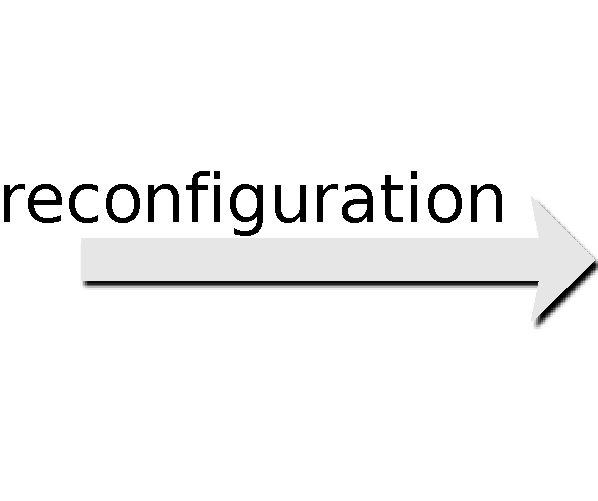
\includegraphics[width=2cm]{img/arrow_reconfiguration}
\end{minipage}
\begin{minipage}[b]{0.40\textwidth}
\begin{lstlisting}
N1: VM1
N2: VM3
N3: VM2 VM4 VM5
N4: VM7 (VM6)
N5: VM8
\end{lstlisting}
\end{minipage}
\caption{A reconfiguration motivated by \cstr{split} constraints.}\label{fig: split}
\end{reconfiguration}


\begin{itemize}

\item \cstr{split(\{\{VM1,VM3\},\{VM2, VM4\}\})}. This constraint was not satisfied in the source configuration as
\cstr{VM2} and \cstr{VM1} were colocated despite they belong to different sets. This violation was fixed
by relocating \cstr{VM2} to \cstr{N3}.

\item \cstr{split(\{\{VM5,VM6\},\{VM7, VM8\}\})}. This constraint was satisfied in the sour\-ce configuration as no set of VMs share hosts. The constraint is still satisfied in the destination configuration: despite \cstr{VM7} and \cstr{VM6} are on the same server, \cstr{VM6} is not in the \st{Running} state, so it is ignored by the constraint.

\end{itemize}

\fullVersion{
\subsection{Model}

The \cstr{split} is modeled by restricting the placement of each d-slice placement variable for
one group to not take any value that is in the other group

\begin{equation*}
\begin{split}
\forall V_1,V_2 \subseteq \mathcal{V} & split(V_1,V_2) \triangleq \\
& \forall v_i \in V_1, v_j \in V_2, d_i^{host} \neq d_j^{host}
\end{split}
\end{equation*}

\subsection{Violation Detection}

The detection of the violating elements in \cstr{split} consists
in computing the sets of used servers for each group of VMs.
The intersection of the two set of servers reveals the misplaced VMs.
This set of VMs is not minimal as only the VMs from one group will have to leave
on each of these server.

\subsection{Availability}

\subsubsection{In {\btrp}}

This constraint in available in {\btrp} since version 2.1.

\begin{equation*}
\begin{split}
\forall V_1,V_2 \subseteq \mathcal{V} & split(V_1,V_2) \triangleq \\
& disjoint(\{d_i, \forall v_i \in V_1\}, \{d_j, \forall v_j \in V_2\})
\end{split}
\end{equation*}
}

\subsection{See also}

\subsubsection{Related Constraints}
\begin{itemize}
\item \cstrref{spread}, \cstrref{lazySpread}: These constraints
disallow the colocation between VMs rather than groups of VMs.
A \cstr{split} constraint is equivalent to a \cstr{lazySpread} constraint when the \cstr{split} constraint is made up with two sets of one VM each.
\item \cstrref{splitAmong}: This constraint forces several set of VMs to be hosted on distinct groups of servers among those explicitly allowed.
\item \cstrref{lonely}. The \cstr{lonely} constraint is a specialization of the \cstr{split} constraint that isolate a set of VMs from all the others. It can then be emulated using a \cstr{split} constraint when the second set of VMs is the absolution complement of the first one.
\end{itemize}

\printListOfInheritance{split}